%==============================================================================
%  REFLEXIVE THEMATIC ANALYSIS  --  CSE 200 Lab Presentation
%  Arafat Bin A Sattar Inan (2305103) | Meherab Hossain (2305108)
%  Dipto Debnath (2305111)
%
%  COMPILE:  pdflatex rta_presentation.tex   (run twice, for the progress bar)
%            or xelatex / lualatex for the full editorial font stack
%==============================================================================
\documentclass[aspectratio=169,11pt,t]{beamer}

%------------------------------------------------------------------ 0. ENGINE
\usepackage{iftex}

%============================== CUSTOM BEAMER THEME ===========================
% (feature 16: custom colours, typography, title page, footer, spacing)

%-- 1. Editorial palette ------------------------------------------------------
\definecolor{paper}   {HTML}{F3EFE6}   % warm ivory background
\definecolor{ink}     {HTML}{202124}   % near-black primary text
\definecolor{mute}    {HTML}{6B6B67}   % muted grey secondary text
\definecolor{plum}    {HTML}{6D597A}   % muted purple
\definecolor{deepblue}{HTML}{355070}   % deep blue
\definecolor{rose}    {HTML}{B56576}   % dusty rose
\definecolor{ochre}   {HTML}{E6A65D}   % ochre
\definecolor{sage}    {HTML}{637E69}   % sage

%-- 2. Typography -------------------------------------------------------------
\ifPDFTeX
  \usepackage[T1]{fontenc}
  \usepackage[utf8]{inputenc}
  \usepackage{charter}                  % Baskerville-like serif for headings
  \usepackage[scaled=0.90]{helvet}      % humanist sans for body text
\else
  \usepackage{fontspec}
  \IfFontExistsTF{Cormorant Garamond}
    {\newfontfamily\headingfont{Cormorant Garamond}}
    {\IfFontExistsTF{Libre Baskerville}
       {\newfontfamily\headingfont{Libre Baskerville}}
       {\newfontfamily\headingfont{Latin Modern Roman}}}
  \IfFontExistsTF{Source Sans 3}
    {\setsansfont{Source Sans 3}}
    {\IfFontExistsTF{Source Sans Pro}{\setsansfont{Source Sans Pro}}{}}
  \IfFontExistsTF{IBM Plex Mono}{\setmonofont{IBM Plex Mono}}{}
\fi
\ifPDFTeX\newcommand{\headingfont}{\rmfamily}\fi

\usepackage{microtype}
\usepackage{array}
\usepackage{booktabs}                   % feature 26: professional tables
\usepackage{amsmath}                    % feature 25: conceptual notation
\usepackage{tikz}
\usetikzlibrary{positioning,calc,arrows,fit,backgrounds,%
                decorations.pathreplacing,overlay-beamer-styles}

\setbeamercolor{background canvas}{bg=paper}
\setbeamercolor{normal text}{fg=ink}
\setbeamercolor{structure}{fg=deepblue}
\setbeamercolor{frametitle}{fg=deepblue}
\setbeamercolor{itemize item}{fg=ochre}
\setbeamercolor{itemize subitem}{fg=mute}

\setbeamerfont{frametitle}{family=\headingfont,size=\LARGE,series=\mdseries}
\setbeamerfont{title}{family=\headingfont,size=\fontsize{30}{34}\selectfont}
\setbeamerfont{subtitle}{size=\normalsize}
\setbeamerfont{itemize/enumerate body}{size=\small}
\setbeamerfont{itemize/enumerate subbody}{size=\footnotesize}

\setbeamertemplate{navigation symbols}{}
\setbeamertemplate{itemize item}{\raisebox{0.12em}{\rule{0.42em}{0.42em}}}
\setbeamertemplate{itemize subitem}{\raisebox{0.18em}{\rule{0.3em}{0.9pt}}}
\setbeamertemplate{section in toc}{%
  \leavevmode\color{deepblue}\inserttocsectionnumber.~\inserttocsection\par}

%-- 3. Frame title: thin ochre rule beneath, generous whitespace --------------
\setbeamertemplate{frametitle}{%
  \vspace*{0.85em}%
  \begin{beamercolorbox}[wd=\paperwidth,leftskip=0.9cm,rightskip=0.9cm]{frametitle}
    {\usebeamerfont{frametitle}\insertframetitle}\\[0.18em]
    {\color{ochre}\rule{2.4cm}{1.1pt}}
  \end{beamercolorbox}%
  \vspace*{-0.2em}
}

%-- 4. Footer: speaker, running title, frame number + progress bar ------------
\newcommand{\currentspeaker}{}
% Total LOGICAL frames across the merged deck (Beamer counts one frame
% per \frame, not per overlay page): Part I=7 + Part II=4 + Part III=7 = 18.
% Used only to keep the footer progress bar proportional after the three
% part-PDFs are merged; each part still numbers and compiles independently.
\newcommand{\decktotalframes}{18}
\setbeamertemplate{footline}{%
  \begin{tikzpicture}[remember picture,overlay]
    \pgfmathsetmacro{\progressfrac}{\insertframenumber/\decktotalframes}
    \fill[mute!30] (0,0.66) rectangle (\paperwidth,0.735);
    \fill[ochre]   (0,0.66) rectangle (\progressfrac\paperwidth,0.735);
    \node[anchor=south west,text=mute,font=\tiny] at (0.9cm,0.16)
         {\textsc{reflexive thematic analysis}};
    \node[anchor=south,text=mute,font=\tiny] at (0.5\paperwidth,0.16)
         {\currentspeaker};
    \node[anchor=south east,text=mute,font=\tiny] at (\paperwidth-0.9cm,0.16)
         {\insertframenumber};
  \end{tikzpicture}%
  \vspace{0.95em}
}

%============================== CUSTOM COMMANDS ===============================
% (feature 17: reusable commands for recurring visual components)

\newcommand{\lede}[1]{{\color{mute}\small #1}\par\medskip}
\newcommand{\term}[1]{{\color{plum}\bfseries #1}}
\newcommand{\hl}[1]{{\color{rose}\bfseries #1}}
\newcommand{\src}[1]{\hfill{\color{mute}\scriptsize #1}}

% Big editorial pull-quote with oversized ochre quotation marks
% (feature 18: custom environment)
\newenvironment{pullquote}[1][]
  {\def\pqsource{#1}%
   \begin{center}\begin{minipage}{0.7\textwidth}
   \setlength{\leftskip}{1.1cm}%
   \noindent\hspace*{-1.1cm}%
   \raisebox{-0.42\height}[0pt][0pt]{%
     \color{ochre}\headingfont\fontsize{56}{56}\selectfont\textquotedblleft}%
   \hspace{0.18cm}%
   \color{ink}\headingfont\fontsize{17}{23}\selectfont\itshape\ignorespaces}
  {\par\vspace{0.5em}%
   \normalfont\footnotesize\color{mute}\hfill--- \pqsource
   \end{minipage}\end{center}}


% Thin-bordered "key idea" panel (feature 21: custom blocks)
\newcommand{\keyidea}[2][deepblue]{%
  \begin{tikzpicture}
    \node[draw=#1,line width=0.8pt,rounded corners=1.5pt,
          inner sep=8pt,text width=0.9\textwidth,align=center,
          font=\small,fill=#1!5] {#2};
  \end{tikzpicture}}

% Member transition slide (feature 17 + smooth hand-overs)
\newcommand{\memberslide}[5]{%
  \begin{frame}[plain]
  \begin{tikzpicture}[remember picture,overlay]
    \coordinate (O) at ([xshift=1.5cm,yshift=-2.1cm]current page.north west);
    \node[anchor=north west,text=ochre,opacity=0.32,
          font=\headingfont\fontsize{95}{95}\selectfont] at (O) {#1};
    \node[anchor=north west,text=mute,font=\scriptsize\sffamily]
          at ([xshift=3.6cm,yshift=-0.15cm]O) {PART #1};
    \node[anchor=north west,text=deepblue,text width=10.5cm,align=left,
          font=\headingfont\fontsize{25}{29}\selectfont]
          at ([xshift=3.6cm,yshift=-0.55cm]O) {#2};
    \draw[ochre,line width=1.4pt]
          ([xshift=3.65cm,yshift=-2.45cm]O) -- ([xshift=6.05cm,yshift=-2.45cm]O);
    \node[anchor=north west,text=ink,font=\normalsize\sffamily\bfseries]
          at ([xshift=3.6cm,yshift=-2.80cm]O) {#3};
    \node[anchor=north west,text=mute,font=\footnotesize\sffamily]
          at ([xshift=3.6cm,yshift=-3.40cm]O) {ID: #4};
    \node[anchor=north west,text=mute,font=\footnotesize\sffamily,
          text width=10.5cm,align=left]
          at ([xshift=3.6cm,yshift=-4.15cm]O) {#5};
  \end{tikzpicture}
  \end{frame}}

%-- Reusable TikZ styles ------------------------------------------------------
% (features 9 & 10: custom nodes + precise positioning)
\tikzset{
  card/.style={draw=mute!50,line width=0.7pt,rounded corners=2pt,
               fill=white,inner sep=7pt,text width=3.5cm,align=left,
               font=\scriptsize},
  phase/.style={circle,draw=deepblue,line width=0.9pt,fill=paper,
                minimum size=1.35cm,align=center,font=\scriptsize,text=ink},
  codebox/.style={draw=sage,line width=0.7pt,fill=sage!12,rounded corners=1.5pt,
                  inner sep=4pt,font=\scriptsize,align=left,text width=3.15cm},
  themebox/.style={draw=plum,line width=1pt,fill=plum!10,rounded corners=2pt,
                   inner sep=6pt,font=\small,align=center,text width=4.1cm},
  flow/.style={->,>=stealth,line width=0.9pt,draw=mute},
  loopback/.style={->,>=stealth,line width=0.8pt,draw=rose,dashed,
                   opacity=0.85,bend right=38},
  tag/.style={font=\tiny\sffamily,text=mute}
}

%==============================================================================
\title{Reflexive Thematic Analysis}
\subtitle{Braun \& Clarke's approach to making meaning from qualitative data}

\date{CSE 200 -- Lab Presentation}

\begin{document}
\setcounter{framenumber}{7} % continues Part I's 7 logical frames

%##############################################################################
\renewcommand{\currentspeaker}{Md. Mehrab Hossain \textperiodcentered\ 2305108}

\memberslide{II}{The six-phase process}{Md. Mehrab Hossain}{2305108}
  {If themes are generated rather than found, what exactly is the work?\\
   Six phases --- they are a loop, not a pipeline.}

%------------------------------------------------ Slide: six phases loop -----
\begin{frame}{Six phases --- and none of them is a one-way street}
\vspace{-1.5em}
\begin{center}
\begin{tikzpicture}[scale=0.90,transform shape]
  % ---- six phases arranged on a circle (feature 10: precise positioning)
  \node[phase,alt=<2>{draw=ochre,line width=1.8pt,fill=ochre!12}{},
        alt=<2->{opacity=1}{opacity=0.18}] (p1) at (90:2.45)   {\textbf{1}\\familiar-\\isation};
  \node[phase,alt=<3>{draw=ochre,line width=1.8pt,fill=ochre!12}{},
        alt=<3->{opacity=1}{opacity=0.18}] (p2) at (30:2.45)   {\textbf{2}\\systematic\\coding};
  \node[phase,alt=<4>{draw=ochre,line width=1.8pt,fill=ochre!12}{},
        alt=<4->{opacity=1}{opacity=0.18}] (p3) at (-30:2.45)  {\textbf{3}\\generating\\themes};
  \node[phase,alt=<5>{draw=ochre,line width=1.8pt,fill=ochre!12}{},
        alt=<5->{opacity=1}{opacity=0.18}] (p4) at (-90:2.45)  {\textbf{4}\\reviewing\\themes};
  \node[phase,alt=<6>{draw=ochre,line width=1.8pt,fill=ochre!12}{},
        alt=<6->{opacity=1}{opacity=0.18}] (p5) at (-150:2.45) {\textbf{5}\\defining \&\\naming};
  \node[phase,alt=<7->{draw=ochre,line width=1.8pt,fill=ochre!12}{},
        alt=<7->{opacity=1}{opacity=0.18}] (p6) at (150:2.45)  {\textbf{6}\\writing\\up};

  % ---- forward arcs
  \draw[flow,visible on=<3->] (p1) to[bend left=18] (p2);
  \draw[flow,visible on=<4->] (p2) to[bend left=18] (p3);
  \draw[flow,visible on=<5->] (p3) to[bend left=18] (p4);
  \draw[flow,visible on=<6->] (p4) to[bend left=18] (p5);
  \draw[flow,visible on=<7->] (p5) to[bend left=18] (p6);

  % ---- recursive feedback arcs (feature 5 + 13)
  \draw[loopback,visible on=<8->] (p3) to (p2);
  \draw[loopback,visible on=<8->] (p4) to (p3);
  \draw[loopback,visible on=<8->] (p4) to[bend right=25] (p2);
  \draw[loopback,visible on=<8->] (p5) to (p4);
  \draw[loopback,visible on=<8->] (p6) to (p5);

  \node[align=center,font=\scriptsize\sffamily,text=mute,visible on=<8->]
       at (0,0.22) {guidelines,\\not rules};
  \node[align=center,font=\tiny\sffamily,text=rose,visible on=<8->]
       at (0,-0.62) {\textsc{recursive}};

  % ---- side commentary panel, changes with the highlighted phase
  \node[anchor=north west,text width=4.5cm,align=left,font=\scriptsize,
        text=ink] at (5,1) {
    \only<1>{Six phases, proposed as a way of \emph{doing} analysis and of
             \emph{learning} to do it.}%
    \only<2>{\term{Phase 1.} Read and re-read. Transcribe yourself if you
             can. Write familiarisation notes. Do not skim.}%
    \only<3>{\term{Phase 2.} Work through the whole dataset, tagging
             anything relevant with short, standalone code labels.}%
    \only<4>{\term{Phase 3.} Cluster codes that share meaning into candidate
             themes. Each needs a central organising concept.}%
    \only<5>{\term{Phase 4.} Test candidates twice --- against the coded
             extracts, then against the whole dataset. Split, merge, or
             discard.}%
    \only<6>{\term{Phase 5.} Write the scope of each theme in two sentences.
             If you cannot, it is not one theme.}%
    \only<7>{\term{Phase 6.} Writing is analysis. It starts at phase one and
             never really stops.}%
    \only<8->{\hl{The arrows go both ways.} Phase four regularly sends you
             back to re-code. Byrne calls the six phases
             ``guidelines, rather than rules''.}};
\end{tikzpicture}
\end{center}
\end{frame}

%---------------------------------- Slide: worked example transformation -----
\begin{frame}{From one sentence of transcript to one theme}
\vspace{-0.6em}
\lede{A worked example, after Byrne (2022): interviews with school teachers
      about promoting student wellbeing.}
\vspace{-0.6em}
\begin{center}
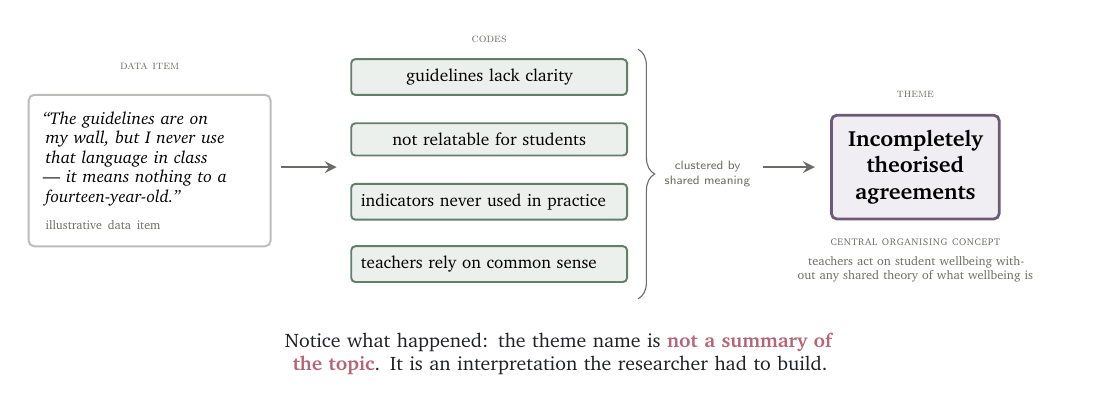
\begin{tikzpicture}[scale=0.88,transform shape]

  %--- stage 1: the data item ------------------------------------------------
  \node[draw=mute!45,line width=0.7pt,fill=white,rounded corners=2pt,
        inner sep=7pt,text width=3.0cm,align=left,font=\scriptsize\itshape,
        alt=<5->{opacity=0.3}{opacity=1}] (data) at (-5.9,0.2)
       {``The guidelines are on my wall, but I never use that language in
         class --- it means nothing to a fourteen-year-old.''\\[3pt]
        \normalfont\tiny\color{mute}illustrative data item};
  \node[tag,alt=<5->{opacity=0.3}{opacity=1}] at (-5.9,1.7) {\textsc{data item}};

  %--- stage 2: the codes ----------------------------------------------------
  \node[tag,visible on=<2->,alt=<5->{opacity=0.3}{opacity=1}] at (-1,2.1)
       {\textsc{codes}};
  \node[codebox,text width = 3.7cm, align = center, visible on=<2->,alt=<5->{opacity=0.3}{opacity=1}]
       (k1) at (-1,1.55) {guidelines lack clarity};
  \node[codebox,text width = 3.7cm, align = center, visible on=<2->,alt=<5->{opacity=0.3}{opacity=1}]
       (k2) at (-1,0.65) {not relatable for students};
  \node[codebox,text width = 3.7cm,visible on=<3->,alt=<5->{opacity=0.3}{opacity=1}]
       (k3) at (-1,-0.25) {indicators never used in practice};
  \node[codebox,text width = 3.7cm,visible on=<3->,alt=<5->{opacity=0.3}{opacity=1}]
       (k4) at (-1,-1.15) {teachers rely on common sense};
   \draw[flow,visible on=<2->] (-4,0.25) -- (-3.2,0.25);

  %--- stage 3: the cluster --------------------------------------------------
  \draw[decorate,decoration={brace,amplitude=6pt},draw=mute,
        visible on=<3->] (1.15,1.95) -- (1.15,-1.65);
  \node[tag,visible on=<3->,text width=1.5cm,align=center] at (2.15,0.15)
       {clustered by shared meaning};

  %--- stage 4: the theme ----------------------------------------------------
  \node[themebox,text width = 2cm,visible on=<4->,
        alt=<5->{draw=plum,line width=1.6pt,fill=plum!18}{}] (th) at (5.15,0.25)
       {\textbf{Incompletely\\ theorised agreements}};
  \node[text width=4.1cm,align=center,font=\tiny,text=mute,visible on=<4->]
       at (5.15,-1.1)
       {\textsc{central organising concept}\\[2pt]
        teachers act on student wellbeing without any shared theory of what
        wellbeing is};
  \node[tag,visible on=<4->] at (5.15,1.3) {\textsc{theme}};
  \draw[flow,visible on=<4->] (2.95,0.25) -- (3.7,0.25);

  %--- closing line ----------------------------------------------------------
  \node[text width=12.4cm,align=center,font=\footnotesize,text=ink,
        visible on=<5->] at (0,-2.45)
       {Notice what happened: the theme name is \hl{not a summary of the
        topic}. It is an interpretation the researcher had to build.};
\end{tikzpicture}
\end{center}
\end{frame}

%----------------------------------------- Slide: code vs theme + revision ---
\begin{frame}{A code is one facet. A theme has many.}
\vspace{-0.3em}
\begin{columns}[T,onlytextwidth]
\begin{column}{0.5\textwidth}
\begin{center}
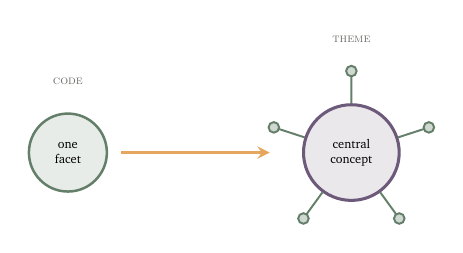
\begin{tikzpicture}[scale=0.9,transform shape]
  \node[tag] at (-2.2,1.9) {\textsc{code}};
  \node[circle,draw=sage,line width=0.9pt,fill=sage!15,minimum size=1.1cm,
        font=\tiny,align=center] at (-2.2,0.9) {one\\facet};
  \node[tag,visible on=<2->] at (1.8,2.5) {\textsc{theme}};
  \node[circle,draw=plum,line width=1.1pt,fill=plum!14,minimum size=1.35cm,
        font=\tiny,align=center,visible on=<2->] (T) at (1.8,0.9)
       {central\\concept};
  \foreach \a in {18,90,162,234,306}
    \draw[sage,line width=0.7pt,visible on=<2->]
      (T) -- ++(\a:1.15) node[circle,fill=sage!30,draw=sage,inner sep=1.5pt]{};
  \draw[->,>=stealth,draw=ochre,line width=1pt,visible on=<2->]
       (-1.45,0.9) -- (0.65,0.9);
\end{tikzpicture}
\end{center}
\vspace{0.2em}
{\footnotesize A theme drawn from a single code is usually still a code.}
\end{column}
\begin{column}{0.42\textwidth}
\vspace{0.4em}
{\small Phase four is where the real work shows.}\\[0.5em]
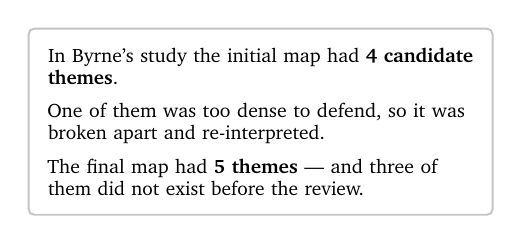
\begin{tikzpicture}
\node[draw=mute!40,line width=0.7pt,rounded corners=2pt,inner sep=7pt,
      text width=5.4cm,font=\scriptsize,align=left,fill=white,
      visible on=<3->]{
  In Byrne's study the initial map had \textbf{4 candidate themes}.\\[4pt]
  One of them was too dense to defend, so it was broken apart and
  re-interpreted.\\[4pt]
  The final map had \textbf{5 themes} --- and three of them did not exist
  before the review.};
\end{tikzpicture}
\vspace{0.5em}

\onslide<4->{\centering{\color{rose}\footnotesize
 Revision is not a sign of failure. It is the method working.}}
\end{column}
\end{columns}
\end{frame}


\end{document}
